\subsubsection{\stid{3.01} hypre} 


\paragraph{Overview} 
The {\sl hypre} software library \cite{hypre,hypre_design_impl_2006} provides high performance preconditioners and solvers for the solution of large sparse linear systems on massively parallel computers, with particular focus on algebraic multigrid solvers. One of {\sl hypre}’s unique features is the provision of a (semi)-structured interface, in addition to a traditional linear-algebra based interface. The semi-structured interface is appropriate for applications whose grids are mostly structured, but with some unstructured features. Examples include block-structured grids, composite grids in structured adaptive mesh refinement (AMR) applications, and overset grids. These interfaces give application users a more natural means for describing their linear systems, and provide access to methods such as structured multigrid solvers, which can take advantage of the additional information beyond just the matrix. Since current architecture trends are favoring regular compute patterns to achieve high performance, the ability to express structure has become much more important. The {\sl hypre} library provides both unstructured and structured multigrid solvers, which have shown excellent scalability on a variety of high performance computers, e.g Blue Gene systems (unstructured solver BoomerAMG has scaled up to 1.25 million MPI cores with a total of 4.5 million hardware threads). It is used by many ECP application teams, including ExaAM, Subsurface, ExaWind, CEED, and more. It requires a C compiler and an MPI implementation, but it also runs in an OpenMP environment. It has some GPU capabilities.
\paragraph{Key  Challenges}

While {\sl hypre}'s solvers contain much parallelism, their main focus is the solution of sparse linear systems, leading to  very large demands on memory bandwidth. In addition, the use of multiple levels, while greatly aiding convergence of the solvers, leads to decreasing systems sizes, number of operations and parallel efficiencies on coarser levels. Particularly the unstructured algebraic multigrid solver BoomerAMG\cite{HeYa2002}, which is {\sl hypre}'s most often used preconditioner, suffers from increasing communication complexities on coarser levels. Coarse grid operators are generated by multiplying three matrices leading to increasing numbers of nonzeroes per row in the resulting matrices and with it increasing numbers of neighbor processes. While BoomerAMG's solve phase mainly consists of matrix vector products and smoothing operations, which are fairly straight forward to parallelize, even on a GPU, its setup phase is highly complex, including many branches, a lot of integer operations as well as some sequential passages. Current  interpolation strategies that lead to best convergence and performance on distributed memory machines are not suitable for implementation on GPUs or similar architectures requiring extreme parallelism. There are several algorithms that are more suitable for GPUs, such as direct interpolation, which however leads to degraded convergence. It could possibly be improved using Jacobi interpolation. All these options would need to be implemented and tested on GPUs. Since {\sl hypre} is a mature product with many solvers and interdependent features, any significant changes that affect the whole library, are tedious and require much testing to ensure that the library stays backward compatible and no features are broken.

\paragraph{Solution Strategy}

Since the upcoming computer architectures are heterogeneous with accelerators, it was very important to enable {\sl hypre} for GPUs. We looked into various options, such as the use of CUDA, OpenMP 4.5, as well as RAJA and Kokkos. We limited the latter two options to the structured interface and solvers which are more natural candidates for such an approach due to their use of macros, called BoxLoops, for loops.
Since computer architectures continue to change rapidly, it is important to come up with strategies that will facilitate future porting of the software. Therefore we decided to develop a new memory model that addresses the use of different memory locations.

\paragraph{Recent Progress}

Under internal LLNL funding we pursued the following ECP-related tasks: enabling portions of several solvers for GPUs, and introducing a new memory model that is based on an abstract machine model.
We  implemented the new memory model as well as 
various GPU capabilities in {\sl hypre}. For the structured solvers, SMG and PFMG\cite{AsFa1996}, both setup and solve phase can now completely be run on GPUs, using both CUDA or OpenMP4.5, and do not require unified memory. In addition, options to use RAJA and Kokkos are available, albeit not well tested yet. 
Porting the unstructured solver, BoomerAMG turned out to be far more complex. Currently only the solve phase can be run on the GPU for select smoothers, mainly Jacobi smoothers, and requires unified memory. The setup phase can currently be performed on the CPU only.

\begin{figure}
\centering
	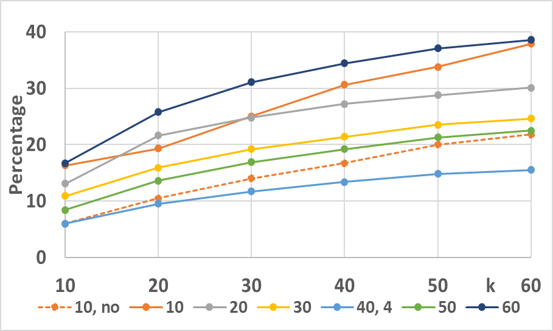
\includegraphics[width=5in]{projects/2.3.3-MathLibs/2.3.3.01-xSDK/COGMRES.png}
	\caption{\label{fig:cogmres} Performance of new GMRES on Vulcan at LLNL}
\end{figure}
`
Under new ECP funding, we implemented a new GMRES solver that has better communication and parallelization properties than the current one and showed improved performance on a BG/Q. 
Figure \ref{fig:cogmres} illustrates the percentage of improvement for increasing the Krylov subspace size k for a 27-point 3D diffusion problem with n x n x n grid points per core using 8192 cores, where n=10, 20, 30, 40, 50, 60. 
For most runs loop unrolling in 8 batches was used, except for `10, no', where none was used to show the effect of saving communication and for n=40, where 4 batches were used. The current implementation is restricted to the CPU, but the solver shows great potential for GPUs. The design of the new solver was a collaboration with the ExaWind team, who demonstrated excellent GPU performance in a paper submitted to Numerical Linear Algebra with Applications \cite{cogmres}. 
We have also started to introduce a new integer datatype called HYPRE$\_$BigInt. The current {\sl hypre} version requires that all integers are converted to 64 bits when solving linear systems greater than 2 billions using the unstructured solvers. The new datatype will allow to only convert variables that need to be 64 bits in that case. This will improve performance and memory usage.

\paragraph{Next Steps}

We will pursue the following tasks:

\begin{itemize}

\item We will finalize the implementation of HYPRE$\_$BigInt and make the new capability available to {\sl hypre} users. 

\item We will continue to add new GPU capabilities to {\sl hypre}. This includes converting various components that are currently running only on the CPU to be usable on the GPU using CUDA or OpenMP 4.5. We will particularly focus on some of the smoothers, e.g. polynomial smoothers, the new GMRES solver, as well as suitable setup kernels. We also plan on improving the efficiency of interfacing applications with {\sl hypre}'s solvers.
\end{itemize}
In addition, we would like to work with ECP application teams who are using {\sl hypre} or would like to use it, to achieve best performance by tuning the solvers for them and potentially implementing suitable algorithmic changes. 


